\documentclass{beamer}

\usefonttheme{serif}

\setbeamertemplate{footline}[frame number]{}
\setbeamertemplate{navigation symbols}{}

\usecolortheme{default}
\setbeamercolor{block title}{bg=lily!20,fg=black}
\setbeamercolor{block body}{bg = blue!10, fg = black}
\setbeamertemplate{itemize item}[square]
\setbeamercolor{itemize item}{fg = cyan}
\setbeamercolor{enumerate item}{fg = cyan}

\usetheme{default}

%\setbeamercolor{titlelike}{fg=black}
%Information to be included in the title page:
\title{Sample title}
\author{Anonymous}
\institute{Overleaf}
\date{2021}

\title[About Beamer] %optional
{Pockels effect}

%\subtitle{A short story}

\author[Arthur, Doe] % (optional, for multiple authors)
{D.~Dedkov }

\institute[VFU] % (optional)
{
	Moscow Institute of Physics and Technology
}

\date[VLC 2023] % (optional)
%{Very Large Conference, April 2021}

%\logo{\includegraphics[height=1cm]{overleaf-logo}}

\begin{document}
	
	\frame{\titlepage}
	
	\begin{frame}
		\frametitle{Abstract}
		TODO
Adjusting screw Scatter plate Analyzer Screen Lazer

$$r_0 \;\; r_1\;\; r_2\;\; ...r_m$$
	\end{frame}
	
	\begin{frame}
		\frametitle{Birefringence}
		%\vspace{-30pt}
		\footnotesize
		In materials refractive index can depend on the polarization and propagation direction of light.
		\begin{figure}
			\footnotesize
			\centering
			\includegraphics[width=0.8\linewidth]{res/birefringence}
			\vspace{-5pt}
			\footnotesize
			\caption{\footnotesize Ordinary ($n_o$) and extraordinary ($n_e$) waves scheme.}
		\end{figure}		
	\end{frame}
	
	\begin{frame}
		\frametitle{Analyzer}

		\begin{figure}
			\centering
			\includegraphics[width=1\linewidth]{res/polarizer_analyzer}
			\caption{Usage of analyzer}
		\end{figure}

		To describe polarization, analyzer and Malus' law is used:
		$$
		I(\theta_i) = I_0 \cos^2{\theta}.
		\label{eq:malus}
		$$
	\end{frame}

		
	\begin{frame}
		\frametitle{Scatter plate}		
		\begin{figure}
			\footnotesize
			\centering
			\includegraphics[width=0.9\linewidth]{res/theta_propagation}
			\vspace{-5pt}
			\footnotesize
			\caption{\footnotesize Ray propogation}
		\end{figure}
		
		\footnotesize
		\begin{itemize}
			\item[] \textbf{Ordinary}: Refractive index stays the same: $n_o(\theta) = n_o$
			
			\item[] \textbf{Extraordinary}: Refractive index can be assumed from:
			
			$$\frac{1}{n_e^2(\theta)} = \frac{\cos^2{\theta}}{n_o^2} + \frac{\sin^2{\theta}}{n_e^2} \implies n_e^2(\theta) \approx n_o - (n_o - n_e) \theta^2$$
		\end{itemize}	
	\end{frame}
	
	\begin{frame}
		\frametitle{Interference observation}
		
		\begin{figure}
			\centering
			\includegraphics[width=1\linewidth]{res/scheme}
			\caption{Experimental setup}
		\end{figure}
		
		Phase shift between ordinary and extraordinary waves can be estimated:
		$$
		\Delta \varphi = \frac{2\pi}{\lambda}l(n_o - n_e)\theta^2,
		$$
		where $\lambda$ -- wavelength, $l$ -- LiNiO$_3$ crystal length.
	\end{frame}

	\begin{frame}
		\frametitle{Conoscopic interference patterns}
		
		\begin{figure}
			\centering
			\includegraphics[width=0.5\linewidth]{res/pattern}
			\caption{Conoscopic interference pattern with the dark "maltese cross"}
		\end{figure}
		
		\footnotesize
		The radius of the nth ring can be calculated by equating: $\Delta \varphi = 2 \pi m$
		$$r^2_m = \frac{\lambda}{l} \frac{(n_o L)^2}{(n_o - n_e)} m,\;\; m = 1,2...,$$
		
		where $L$ -- distance from crystal to the screen.
	\end{frame}
		
	\begin{frame}[plain,c]	
		\begin{center}
			\huge \usebeamercolor[fg]{frametitle} Measurements and Results
		\end{center}
	\end{frame}	
	
	\begin{frame}
		\frametitle{Experimental Setup}
		
		\begin{figure}
			\centering
			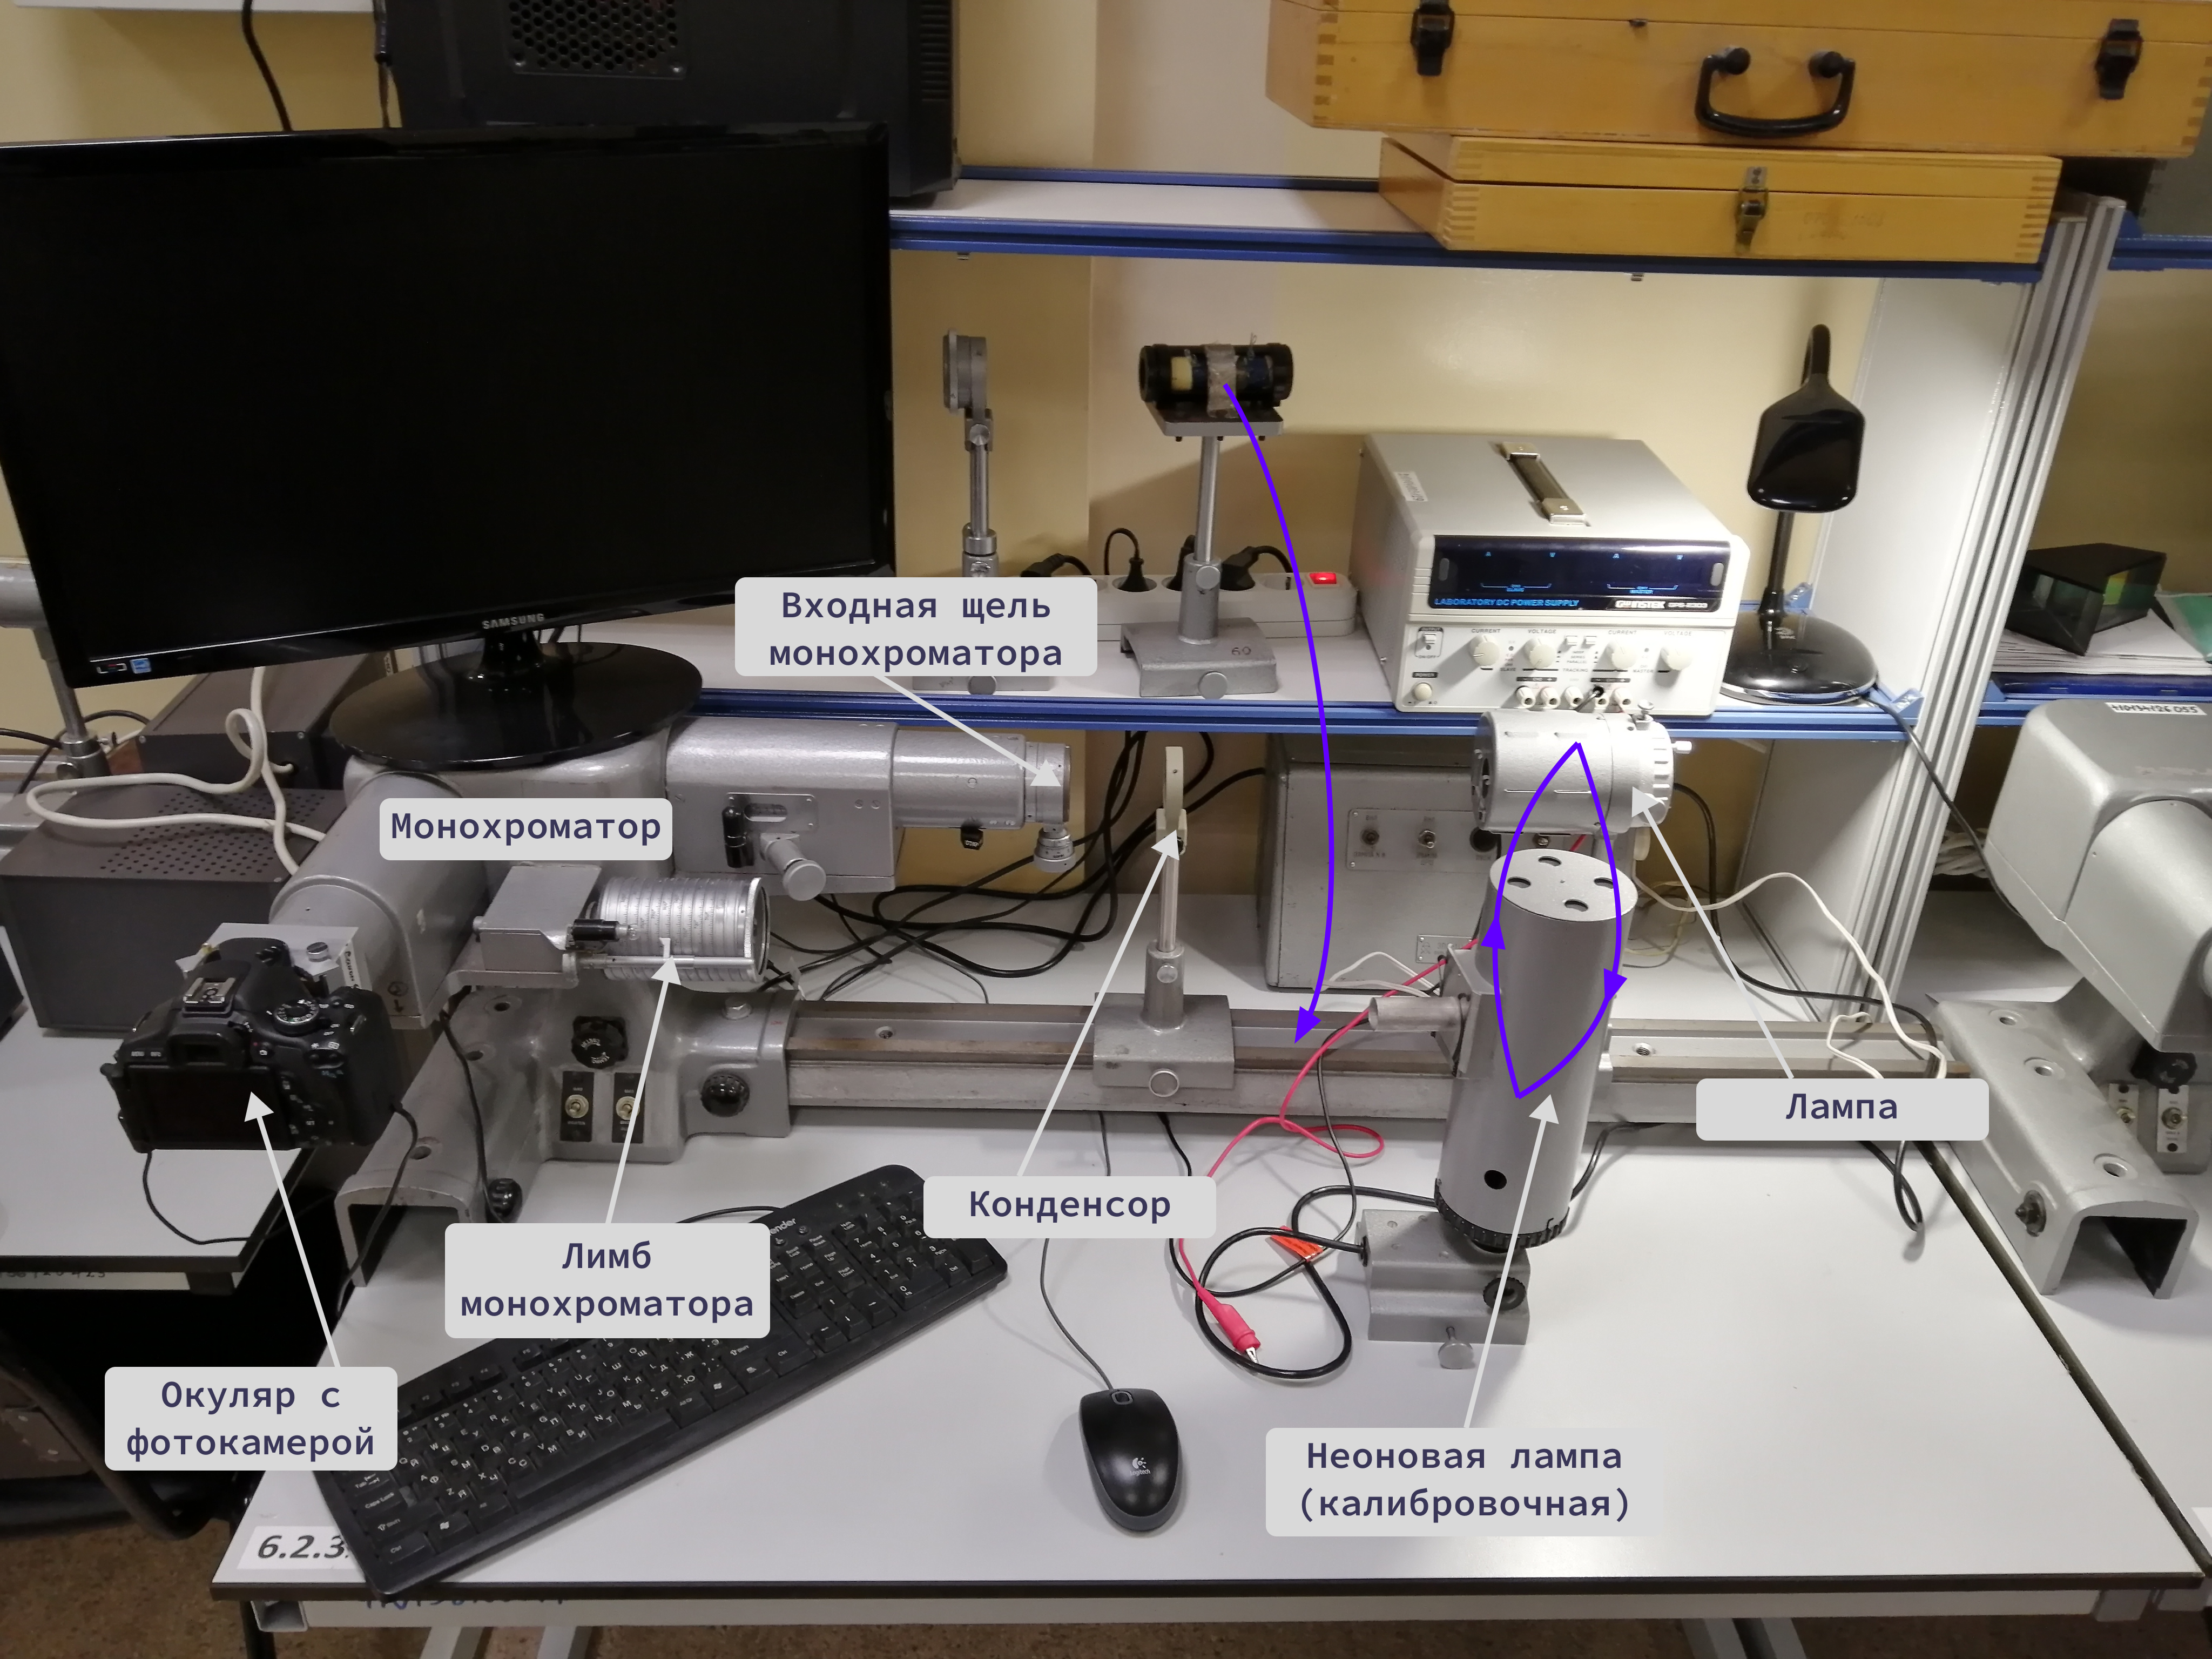
\includegraphics[width=1\linewidth]{res/setup.png}
			\caption{Photo of laboratory setup}
		\end{figure}
	\end{frame}
	
	\begin{frame}
		\frametitle{Population inversion}		
		\begin{columns}
			\footnotesize
			\begin{column}{0.6\textwidth}
				\begin{figure}
					\footnotesize
					\centering
					\includegraphics[width=1\linewidth]{res/metastable}
					\vspace{-5pt}
					\footnotesize
					\caption{\footnotesize Energy levels of $Er3+$ ions in quartz glass}
				\end{figure}
			\end{column}
			\begin{column}{0.5\textwidth}
				Gain: 
				$$\gamma =  N_2\sigma_{21}(\lambda) -  N_1\sigma_{12}(\lambda)$$
				
				\begin{itemize}
					\item[$1480$ nm] Quasi-two-level system: spectral lines $4I_{13/2}, 4I_{15/2}, 4I_{11/2}$ are split due to the Stark effect. Then $\sigma_{12}(\lambda) \neq \sigma_{21}(\lambda)$.
					
					\item[$980$ nm] Three-level system. Has a high efficiency, but generates more noise.
				\end{itemize}				
			\end{column}
		\end{columns}	
	\end{frame}
	
	\begin{frame}
		\frametitle{Optical Signal to Noise Ratio}

		\includegraphics[width=0.80\linewidth]{res/osnr}
		\footnotesize
		
		OSNR compares the level of a desired signal to the level of background noise:
		$$F = \frac{\text{OSNR}_{\text{in}}}{\text{OSNR}_{\text{out}}}$$
		$$NF = 10\log{\left(F\right)} = \text{osnr}_{\text{in}} - \text{osnr}_{\text{out}}$$		
	
	\end{frame}

\begin{frame}
	\frametitle{Feedback mechanism}
	\includegraphics[width=1\linewidth]{res/isolator}
	\footnotesize
	The process of continuous laser generation turns the amplifier into a laser and completely destroys the structure of the input signal. Avoid optical feedback by introducing \textbf{optical isolators} into the system.
\end{frame}

\begin{frame}
	\frametitle{Quantum OSNR}
	\includegraphics[width=0.9\linewidth]{res/spontanious_emission}
	
	\footnotesize
	When the source signal doesn't have amplified spontaneous emission we can estimate quantum signal-to-noise ratio (SNR) using the Heisenberg uncertainty principle:
	
	$$\text{OSNR}_{\text{in}}^Q = \frac{P_{\text{in}}}{h \nu \Delta\nu}$$

	Hence:
	$$\text{NF} = -10\log{(h \nu \Delta\nu)} + P_{\text{in}} - \text{osnr}_{\text{out}}$$
	
\end{frame}

\begin{frame}
	\frametitle{Gain}
	\begin{figure}
		\footnotesize
		\centering
		\includegraphics[width=1\linewidth]{res/theory_gain}
		\vspace{-5pt}
		\footnotesize
		\caption{\footnotesize Small-signal gain as a function of (a) pump power and (b) amplifier length for an EDFA. }
	\end{figure}

	The central EDFA criteria is gain:
	$$G = \frac{P_{\text{in}}}{P_{\text{out}}}$$

\end{frame}


	
\begin{frame}
	\frametitle{Feedback mechanism}
	
	
	$$\lambda = 980 \text{ or } 1480\; \text{nm}$$
	
	$$\tau \sim 10 \text{ms} \;\;\; \tau \sim 1 \text{us}$$
	
	$$N_1 \; N_2 \; \sigma_{21}(\lambda) \; \sigma_{12}(\lambda) \;$$
	
	$$4I_{13/2} \;\; 4I_{15/2}\;\; 4I_{11/2}$$
	
	wavelength, nm power, dBm $p_{\text{spon}} = 10\log{\left(P_{\text{spon}}\right)}\;\; P_{\text{stim}} \;\; p_{\Sigma} = 10\log{\left(P_{\text{spon}} + P_{\text{stim}} \right)} $
	dB
\end{frame}

	
\end{document}